\documentclass[12pt]{article}

\usepackage{graphicx}
\usepackage{amsmath}
\usepackage{amssymb}
\usepackage{natbib}
\usepackage{amsfonts}
\usepackage{multicol}
\usepackage{float}
\usepackage{oldgerm}
\usepackage{bm}
\usepackage{mathtools}
\usepackage{wrapfig}
\usepackage{fancyhdr}
\usepackage[export]{adjustbox}
\usepackage{xcolor}

\pagestyle{empty}

\newcommand{\Avec}{\mathbf A}
\newcommand{\Bvec}{\mathbf B}
\newcommand{\Dvec}{\mathbf D}
\newcommand{\Evec}{\mathbf E}
\newcommand{\Fvec}{\mathbf F}
\newcommand{\Jvec}{\mathbf J}
\newcommand{\Lvec}{\mathbf L}
\newcommand{\Mvec}{\mathbf M}
\newcommand{\Pvec}{\mathbf P}
\newcommand{\Svec}{\mathbf S}
\newcommand{\avec}{\mathbf a}
\newcommand{\bvec}{\mathbf b}
\newcommand{\dvec}{\mathbf d}
\newcommand{\evec}{\mathbf e}
\newcommand{\fvec}{\mathbf f}
\newcommand{\jvec}{\mathbf j}
\newcommand{\kvec}{\mathbf k}
\newcommand{\nvec}{\mathbf n}
\newcommand{\pvec}{\mathbf p}
\newcommand{\rvec}{\mathbf r}
\newcommand{\svec}{\mathbf s}
\newcommand{\vvec}{\mathbf v}
\newcommand{\xvec}{\mathbf x}
\newcommand{\yvec}{\mathbf y}
\newcommand{\zvec}{\mathbf z}
\newcommand{\nablav}{\boldsymbol{\nabla}}
\newcommand{\nablavector}{\vec \nabla}
\newcommand{\alphavec}{\boldsymbol{\alpha}}
\newcommand{\phivec}{\boldsymbol{\phi}}
\newcommand{\thetavec}{\boldsymbol{\theta}}
\newcommand{\omegavec}{\boldsymbol{\omega}}
\newcommand{\tauvec}{\boldsymbol{\tau}}
\newcommand{\ezero}{\varepsilon_{0}}
\newcommand{\mzero}{\mu_{0}}
\newcommand{\mubold}{\boldsymbol{\mu}}
\newcommand{\uniti}{\hat{\boldsymbol{\imath}}}
\newcommand{\unitj}{\hat{\boldsymbol{\jmath}}}
\newcommand{\unitk}{\hat{\boldsymbol{\mathit{k}}}}
\newcommand{\unitn}{\hat{\mathbf n}}
\newcommand{\unitr}{\hat{\mathbf r}}
\newcommand{\unitphi}{\hat{\boldsymbol{\phi}}}
\newcommand{\unittheta}{\hat{\boldsymbol{\theta}}}

\newcommand{\bit}{\begin{itemize}}
\newcommand{\eit}{\end{itemize}}

\setlength{\headsep}{0.5cm}
\setlength{\oddsidemargin}{-0.5cm}
\setlength{\textwidth}{16.5cm}
\setlength{\textheight}{24cm}
\voffset = -2cm

\pagestyle{fancy}
\fancyhf{}
\rfoot{
\includegraphics[width=1.0in]{cnm.png}}
\lfoot{ENGR 2910 Homework 8}
\begin{document}

%{\bf \underline{STUDENT NAME}:} 
%\vspace{1cm}

\begin{center}
\hfil
%\begin{wrapfigure}{l}{0.5in} 
%    
\includegraphics[width=0.5in]{cnm.png}
%\end{wrapfigure}
{\large\bf {ENGR 2910-101: Circuit Analysis}}
\hfill Instructor: Leo Silbert \\
Homework 8: 10/27/21 \hfill Due: 11/03/20\\
\hrulefill\\
\end{center}

%{\em Show all your working to ensure you obtain full points. Partial
%  credit will be given for correct algebraic steps if you fail to
%  obtain the correct final answer.}\\

%\newpage


\noindent
{\bf Question 1} [10]

Use the mesh-current method to find $v_{1}$ and $v_{2}$ in the circuit below.
\begin{figure}[h!]
     \centering
\vspace{-0.1in}
     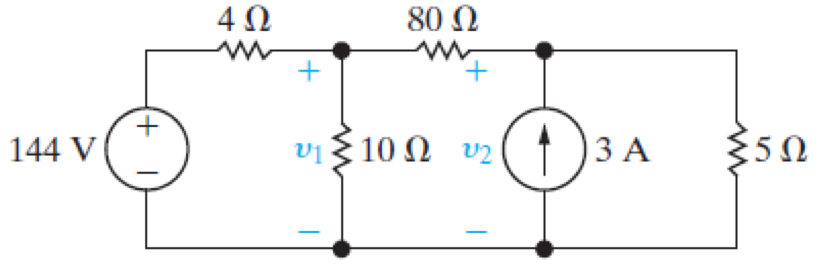
\includegraphics[clip,width=0.7\textwidth]{Fig4-11.png}
\vspace{-0.15in}
\end{figure}


\noindent
{\bf Question 2} [10]

Use the mesh-current method to find the total power developed by the three indepedent voltage sources. Also, explcitly evaluate the power dissipated in the 6 resistors to double check your calculation.
\begin{figure}[h!]
     \centering
\vspace{-0.1in}
     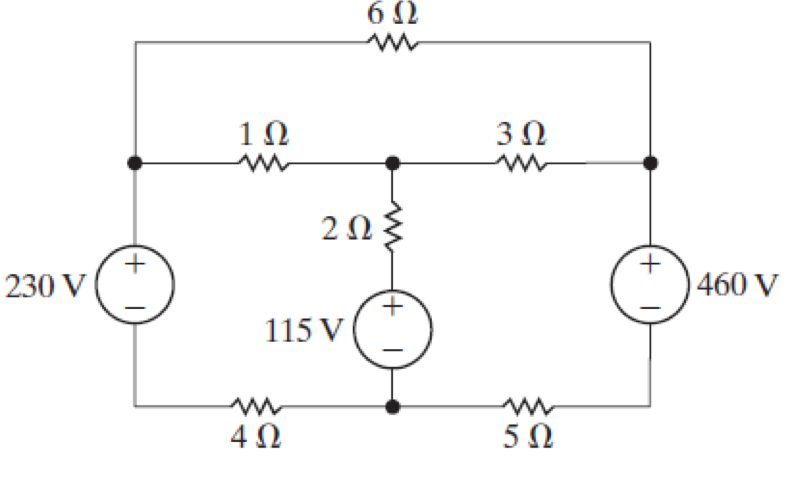
\includegraphics[clip,width=0.7\textwidth]{Fig4-37.png}
\vspace{-0.15in}
\end{figure}

\noindent
{\bf Question 3} [10]

Use the mesh-current method to find the power developed in the three voltage sources.
\begin{figure}[h!]
  \centering 
  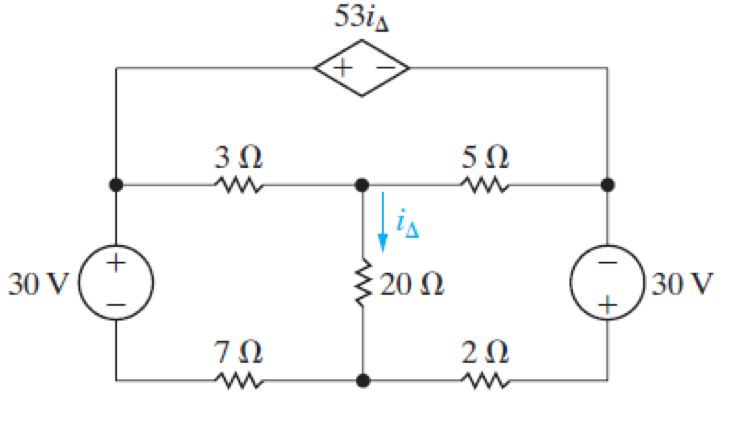
\includegraphics[clip,width=0.6\textwidth]{Fig4-40.png}
\end{figure}

\newpage
\noindent
{\bf Question 4} [10]

Use the mesh-current method to determine which of the three sources is providing power to the circuit and which are absorbing power. What are the values of the power in each case? Go on to then compute the power dissipated in the resistors to ensure power conversation. 
\vspace{0.1in}
\begin{figure}[h]
  \centering 
  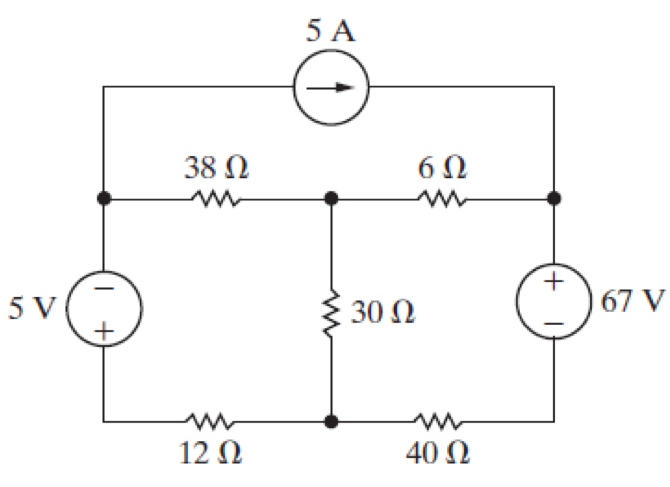
\includegraphics[clip,width=0.6\textwidth]{Fig4-45.png}
\end{figure}

\vspace{0.1in}
\noindent
{\bf Question 5} [10]

Use the mesh-current method to find the three branch currents identified in the circuit below. [Hint: identify the supermesh.]
\begin{figure}[h!]
\centering 
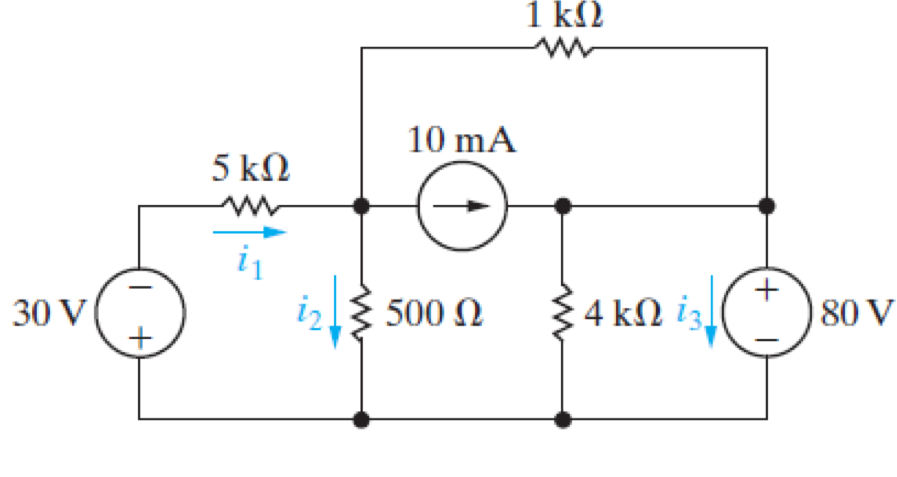
\includegraphics[clip,width=0.8\textwidth]{Fig4-23.png}
\end{figure}


\end{document}
